%\begin{figure}[!ht]
%  \centering
%  \begin{tikzpicture}
%    \draw[very thin, gray] (0,2) grid (1,3);
%    \draw[very thin, gray] (0,1) grid (3,2);
%    \draw[very thin, gray] (0,0) grid (5,1);
%    \draw[fill=black!20] (0,0) rectangle (1,1);
%
%    \foreach \i\j in {0/1,1/1,2/1,3/1,4/3}{
%      \node at (\i+0.5, 0.5) {\j};
%    }
%
%    \foreach \i\j in {0/2,1/3,2/3}{
%      \node at (\i+0.5, 1.5) {\j};
%    }
%
%    \node at (0.5,2.5) {5};
%  \end{tikzpicture}
%  \caption{Example of tableau}
%  \label{fig:example_tableau}
%\end{figure}
%
%\begin{figure}[!h]\centering
%  
% \experiment{
%    \procedure[space = auto]{patati}{%
%      \pcif \mathsf{p} = \top\\
%      \pcelse \\
%      \pcreturn \bot\\
%      \pcfi
%    }
%  }
%  \label{alg1}
%  \caption{nice algo}
%\end{figure}

\section{Présentation} \label{sect1.1}
Pour comprendre ce qu'est le monoïde plaxique, commençons par définir ce qu'est un monoïde. 
\begin{definition}[Monoide] \label{def:monoid}
  Il s'agit d'une structure algébrique possédant une loi interne associative et un élément neutre.
\end{definition}
Autrement dit, c'est un ensemble $E$ qui possède une loi que nous appellerons multiplication et noterons $\times$. L'associativité nous dit que si on multiplie plus de deux éléments, l'ordre dans lequel on effectue les multiplications n'a pas d'importance. 
\begin{remark}
  Un monoïde n'est en général pas commutatif : si $x,y \in E$, on n'a pas nécessairement $x \times y = y \times x$.
\end{remark}
\begin{property} \label{prop:commut}
  En particulier, le monoïde plaxique n'est pas commutatif.
\end{property}

Avant de définir le monoïde plaxique, il nous faut présenter d'autres objets : les tableaux de Young. Il existe plusieurs manières équivalentes de les définir, et nous reprenons ici celle de Chris Monico dans~\cite{monico2022division}. 

Soit $\AN$ un ensemble ordonné de $N$ symboles (un alphabet ordonné). Dans ce rapport, pour simplifier l'écriture, nous utiliserons $\AN = \{1,2,...,N\}$.
\begin{definition}[fermeture de Kleene]
  La fermeture de Kleene $\A$ de l'alphabet $\AN$ est l'ensemble des mots de longueur finie formés de lettres de $\AN$ (y compris le mot vide).
\end{definition}

Pour un mot $m \in \A$, nous noterons $|m|$ sa longueur (le nombre de lettres qu'il contient) et $m_i$ le $i$-ème symbole dans le mot. On a donc $m=m_1m_2...m_{|m|}$.

\begin{definition}[tableau] \label{def:tab}
  Un tableau de Young semi-standard sur $\AN$ (que nous appellerons abusivement dans la suite tableau de Young ou simplement tableau) est une suite finie $T=(L_1,L_2,...,L_N)$ de mots sur $\A$ (potentiellement vides) respectant les contraintes suivantes : 
  \begin{enumerate}
    \item $|L_1| \geq |L_2| \geq ... \geq |L_N|$
    \item Dans chaque mot $L_i$, les symboles apparaissent dans l'ordre croissant
    \item Pour tout $i \in [\![1;N-1]\!]$, pour tout $j \in [\![1;|L_{i+1}|]\!]$, $(L_{i+1})_j > (L_i)_j$
  \end{enumerate}
\end{definition}

On représente un tableau sous la forme suivante : \\
\begin{figure}[!ht]
  \centering
  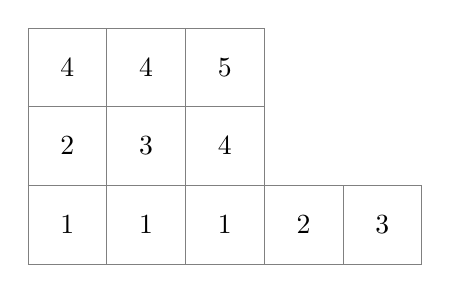
\begin{tikzpicture}
    \draw[very thin, gray] (0,2) grid (3,3);
    \draw[very thin, gray] (0,1) grid (3,2);
    \draw[very thin, gray] (0,0) grid (5,1);
    \foreach \i\j in {0/1,1/1,2/1,3/2,4/3}{
      \node at (\i+0.5, 0.5) {\j};
    }

    \foreach \i\j in {0/2,1/3,2/4}{
      \node at (\i+0.5, 1.5) {\j};
    }

    \foreach \i\j in {0/4,1/4,2/5}{
      \node at (\i+0.5, 2.5) {\j};
    }
    
  \end{tikzpicture}
  \caption{Exemple de tableau}
  \label{fig:tab1}
\end{figure}
\\
\vspace*{-2em} \noindent Ici on a donc $L_1=11123$, $L_2=234$ et $L_3=445$.

\vspace*{2em}
Avec cette représentation, on peut reformuler les contraintes de la façon suivante : en lisant le tableau de gauche à droite et de bas en haut,
\vspace*{-1em}
\begin{enumerate}[parsep=0cm, itemsep=0cm]
	\item les lignes sont de longueur décroissante
	\item les symboles sont croissants sur les lignes
	\item les symboles sont strictement croissants sur les colonnes
\end{enumerate}

\begin{remark}
  Certains auteurs écrivent les tableaux dans l'autre sens (avec la ligne la plus longue en haut et la plus courte en bas). La notation que nous utilisons est appelée notation française, et l'autre notation anglaise.
\end{remark}

On définit la lecture par ligne d'un tableau $T=(L_1,...,L_N)$ par 
\begin{definition}[lecture par ligne] \label{def:row_reading}
  $\rho(T)=R_NR_{N-1}...R_1$ (concaténation des lignes de haut en bas). 
\end{definition} \vspace*{-1em}
\noindent Par exemple, si on prend $T$ le tableau représenté en \ref{fig:tab1}, $\rho(T)=44523411123$

L'algorithme de Schensted~\cite{schensted1961longest} permet de construire un tableau à partir d'un mot. Le principe est le suivant : on commence avec un tableau vide. A chaque étape, on reprend le tableau obtenu à l'étape précédente en y insérant la première lettre du mot et on enlève la première lettre du mot. On recommence jusqu'à ce que le mot soit vide. L'insertion se fait de telle sorte qu'à chaque étape le tableau vérifie toutes les contraintes. Nous la détaillerons dans le chapitre~\ref{ch2}. On note $P(m)$ le tableau ainsi construit à partir du mot $m$.

La fonction $P$ de $\A$ dans l'ensemble des tableaux de Young semi-standards n'est pas injective. C'est-à-dire que deux mots différents peuvent être représentés par le même tableau. Cependant, Knuth \cite{knuth1970permutations} a trouvé une relation d'équivalence sur $\A$, appelée équivalence de Knuth caractérisant les mots ayant la même image par $P$. L'équivalence de Knuth que nous noterons $\equiv$ est générée par les relations suivantes : 
\begin{definition}[Relations de Knuth] \label{def:rel_knuth}
  Pour tous $a,b,z \in \AN$, $$\text{si min}\{a,b\}<z\leq\text{max}\{a,b\}\text{ alors }zab \equiv zba$$ $$\text{si min}\{a,b\}\leq z<\text{max}\{a,b\}\text{ alors }abz \equiv baz$$
\end{definition}

\medskip
\begin{definition}[monoïde plaxique] \label{def:monoide_plaxique}
  On définit alors le monoïde plaxique comme étant l'ensemble quotient $\P=\A/\equiv$. 
\end{definition}
On note $[m]$ la classe d'équivalence d'un mot $m$ dans $\A$. Knuth a prouvé dans~\cite{knuth1970permutations} que $P(u)=P(v)$ si et seulement si $[u]=[v]$, i.e si et seulement si $u \equiv v$. De plus, nous avons $P(\rho(T))=T$ pour tout tableau $T$. Le représentant canonique de chaque classe $[u] \in \P$ sera donc naturellement $\rho(P(u))$.

Rigoureusement, un élément du monoïde plaxique sur $\A$ est donc une classe d'équivalence $[u]$ de mots de $\A$. On pourra confondre cette classe avec le tableau $P(u)$ puisque la fonction $P$ de $\P$ dans l'ensemble des tableaux semi-standards est bijective (ce qui signifie qu'à tout élément de $\P$ on peut associer un unique tableau via la fonction $P$, et vice-versa).

Il existe une opération sur l'ensemble des tableaux nommée multiplication de Knuth. Cette opération que nous détaillerons dans la partie \ref{subsect:mult} se base sur l'algorithme de Schensted. Il s'agit d'une loi interne associative admettant pour élément neutre le tableau vide, faisant de $\P$ un monoïde. Cette multiplication n'est pas commutative.

Dans ce rapport, nous appellerons tout opérateur vérifiant la propriété suivante opérateur de division : 
\begin{definition}[division]
  Un opérateur binaire $/$ est un opérateur de division (à droite) sur un ensemble $E$ si et seulement si pour tous $a,b \in E$, $((ab)/b)b=ab$
\end{definition}

Dans $\P$, tous les éléments ne sont pas divisibles. Cependant, pour une application cryptographique, tous les éléments que nous diviserons auront été construits à partir d'une multiplication et seront donc divisibles. Il n'y a pas non plus unicité de la solution à une division : il est possible que des tableaux $a,b,d,q$  avec $a \neq q$, on ait $ab=c$ et $qb=c$ : on dit que $\P$ n'est pas régulier.

Les algorithmes de divisions présentés dans ce rapport essaieront donc de résoudre le problème suivant : 
\begin{problem} \label{prob:div}
  Pour $[b], [c] \in \P$, trouver $[q] \in \P$ telle que $[q][b]=[c]$, sachant qu'une telle classe $[q]$ existe.
\end{problem}

\section{Application à la cryptographie}
Dans la majorité des cas, lorsque deux personnes ou machines communiquent, il est souhaitable que les messages puissent être lu uniquement par  leur destinataire. Cependant, quel que soit le canal utilisé, il est toujours possible pour une personne mal intentionnée d'intercepter les messages et de les lire. C'est là qu'intervient la cryptographie: elle a pour but de s'assurer que si une personne reçoit un message qui ne lui est pas destiné, elle ne puisse pas l'interpréter. Les méthodes de chiffrement font usage d'une clé connue uniquement de l'émetteur et du destinataire qui permet de chiffrer et déchiffrer les messages. L'inconvénient de cette méthode est qu'il faut trouver un moyen sécurisé de s'échanger la clé.

Pour palier à ce problème, des algorithmes de cryptographie asymétrique tel que le chiffrement RSA~\cite{rivest1978method} ont été inventés. Avec cet algorithme, chaque communicant possède 2 clés : une clé publique (connue de tous) pour le chiffrement et une clé privée (connue du destinataire seulement) pour le déchiffrement. La création des clés utilise des propriétés des nombres premiers, et la sécurité de l'algorithme tient au fait que si on choisit 2 grands nombres premiers et qu'on les multiplie, il est à l'heure actuelle impossible de factoriser le résultat en un temps raisonnable. Le fait de prendre deux nombres premiers et de les multiplier est en revanche très rapide. Cependant, en 1994, Peter Shor publia un algorithme quantique~\cite{Shor} qui factorise un entier en un temps polynomial et qui permettrait donc, s'il était implémenté, de calculer la clé privée à partir de la clé publique pour le RSA. En 2023, les ordinateurs quantiques ne sont encore pas assez perfectionnés pour utiliser l'algorithme sur de grands nombres, mais il est probable que cela pose problème dans le futur.

L'un des enjeux actuels de la recherche en sécurité est donc de trouver de nouvelles méthodes pour générer des clés qui ne résisteraient à l'algorithme de Shor. Dans~\cite{Brown+2023}, Daniel R. L. Brown propose une méthode utilisant le monoïde plaxique. La sécurité de cette méthode repose sur le fait qu'il semble difficile (au sens ou cela prend beaucoup de temps) de diviser un élément de ce monoïde par un autre. C'est pourquoi nous avons porté notre attention sur l'étude des algorithmes de division dans ce monoïde.

\section{Le monoïde plaxique dans la littérature}

\subsection{Historique du monoïde plaxique}
Le monoïde plaxique est définie pour la première fois en 1970 par Donald Knuth dans~\cite{knuth1970permutations}. Il définit dans son article l'algèbre de monoïde du monoïde plaxique sur l'anneau des entiers qu'il appelle l'algèbre des tableaux. Pour cela, il a utilisé l'algorithme de Schensted dont nous avons déjà parlé pour associé les éléments du monoïde plaxique à des tableaux de Young. Les Tableaux de Young ont quant à eux été introduits en 1900 par Alfred Young, mathématicien à l'université de Cambridge~\cite{young1900quantitative}. Les tableaux de Young ont plusieurs applications, mais nous ne les détaillerons pas car notre étude porte uniquement sur le monoïde plaxique.

Le nom de monoïde plaxique a été donné par Lascoux et Schützenberger~\cite{lascoux1981monoide}. 

\subsection{Pour une application cryptographique} \label{etat_recherche}
Brown pré-publie en 2021 sur le site Cryptology ePrint Archive un article intitulé Plactic key agreement (insecure?)~\cite{brown2021plactic}. Cet article a été publié en 2023 dans le Journal of Mathematical Cryptology~\cite{Brown+2023}. Brown y présente un nouveau protocole d'échange de clés utilisant le monoïde plaxique nommé échange de clés plaxique. D'après lui, ce  protocole pourrait avoir des applications pratiques si les 2 conjectures suivantes étaient vérifiées (sur un alphabet d'au moins 64 symboles) : 
\begin{conjecture} \label{conj:brown1}
  L'érosion est l'algorithme de division le plus rapide dans le monoïde plaxique.
\end{conjecture}
\begin{conjecture} \label{conj:brown2}
  Pour calculer $d/b$ avec $|b|=L$ et $|d|=2L$, l'érosion a un coût moyen d'au moins $2^{L^{0.81}}$. Plus précisément, la moyenne du logarithme en base 2 du coût est approximativement $L^{0.81}$. De plus, ces logarithmes de coût sont distribués suivant une loi normale d'écart type $1/8$ fois la moyenne.
\end{conjecture}
La conjecture \ref{conj:brown2} est issue d'observations empiriques faites sur des mots générés aléatoirement.

La conjecture \ref{conj:brown1} est la plus importante car la seconde n'a plus d'intérêt si elle se révélait fausse. Au début de notre projet, notre but était d'étudier, comparer et implémenter les différents algorithmes présentés par Brown dans l'optique de chercher un algorithme plus performant. Cependant, en décembre 2022 Chris Monico pré-publia un article~\cite{monico2022division} décrivant un nouvel algorithme de division beaucoup plus rapide que l'érosion. Notre projet a alors changé de direction : nous nous sommes attachés à comprendre, implémenter et tester les algorithmes de Monico afin de reproduire ses résultats.

L'algorithme de Monico est un algorithme probabiliste dont il est très compliqué de calculer la complexité. Il serait donc intéressant de trouver un algorithme déterministe dont on pourrait calculer la complexité afin de connaitre de manière certaine le temps qu'il faudrait pour effectuer une division.

Dans la version non publiée de son article, Brown propose un challenge qui consiste à trouver une solution à un mot de taille 1024 par un mot de taille 512 sur un alphabet de taille 64, qui serait en pratique insolvable avec la division par érosion. Avec son algorithme, Monico trouva une solution en 503 secondes.